% THIS DOCUMENT IS FOLLOWS THE VOLERE TEMPLATE BY Suzanne Robertson and James Robertson
% ONLY THE SECTION HEADINGS ARE PROVIDED
%
% Initial draft from https://github.com/Dieblich/volere
%
% Risks are removed because they are covered by the Hazard Analysis
\documentclass[12pt]{article}

\usepackage{booktabs}
\usepackage{tabularx}
\usepackage{graphicx}
\usepackage{hyperref}
\hypersetup{
    bookmarks=true,         % show bookmarks bar?
      colorlinks=true,      % false: boxed links; true: colored links
    linkcolor=red,          % color of internal links (change box color with linkbordercolor)
    citecolor=green,        % color of links to bibliography
    filecolor=magenta,      % color of file links
    urlcolor=cyan           % color of external links
}

\newcommand{\lips}{\textit{Insert your content here.}}

%% Comments

\usepackage{color}

\newif\ifcomments\commentstrue %displays comments
%\newif\ifcomments\commentsfalse %so that comments do not display

\ifcomments
\newcommand{\authornote}[3]{\textcolor{#1}{[#3 ---#2]}}
\newcommand{\todo}[1]{\textcolor{red}{[TODO: #1]}}
\else
\newcommand{\authornote}[3]{}
\newcommand{\todo}[1]{}
\fi

\newcommand{\wss}[1]{\authornote{blue}{SS}{#1}} 
\newcommand{\plt}[1]{\authornote{magenta}{TPLT}{#1}} %For explanation of the template
\newcommand{\an}[1]{\authornote{cyan}{Author}{#1}}

%% Common Parts

\newcommand{\progname}{Course Buddy} % PUT YOUR PROGRAM NAME HERE
\newcommand{\authname}{Team \#5, Overwatch League
\\ Jingyao, Qin
\\ Qianni, Wang
\\ Qiang, Gao
\\ Chenwei, Song
\\ Shuting, Shi
\\ } % AUTHOR NAMES                  

\usepackage{hyperref}
    \hypersetup{colorlinks=true, linkcolor=blue, citecolor=blue, filecolor=blue,
                urlcolor=blue, unicode=false}
    \urlstyle{same}
                                

\begin{document}

\title{Software Requirements Specification for \progname: subtitle describing software} 
\author{\authname}
\date{\today}
	
\maketitle
~\newpage

\pagenumbering{roman}

\tableofcontents

~\newpage

\section*{Revision History}

\begin{tabularx}{\textwidth}{p{3cm}p{2cm}X}
\toprule {\textbf{Date}} & {\textbf{Version}} & {\textbf{Notes}}\\
\midrule
Date 1 & 1.0 & Notes\\
Date 2 & 1.1 & Notes\\
\bottomrule
\end{tabularx}

~\\

~\newpage
\section{Purpose of the Project}
\subsection{User Business}
\lips
\subsection{Goals of the Project}
\lips
\section{Stakeholders}
\subsection{Client}
\lips
\subsection{Customer}
\lips
\subsection{Other Stakeholders}
\lips
\subsection{Hands-On Users of the Project}
\lips
\subsection{Personas}
\lips
\subsection{Priorities Assigned to Users}
\lips
\subsection{User Participation}
\lips
\subsection{Maintenance Users and Service Technicians}
\lips

\section{Mandated Constraints}
\subsection{Solution Constraints}
\lips
\subsection{Implementation Environment of the Current System}
\lips
\subsection{Partner or Collaborative Applications}
\lips
\subsection{Off-the-Shelf Software}
\lips
\subsection{Anticipated Workplace Environment}
\lips
\subsection{Schedule Constraints}
\lips
\subsection{Budget Constraints}
\lips
\subsection{Enterprise Constraints}
\lips

\section{Naming Conventions and Terminology}
\subsection{Glossary of All Terms, Including Acronyms, Used by Stakeholders
involved in the Project}
\lips

\section{Relevant Facts And Assumptions}
\subsection{Relevant Facts}
\lips
\subsection{Business Rules}
\lips
\subsection{Assumptions}
\lips

\section{The Scope of the Work}
\subsection{The Current Situation}
\lips
\subsection{The Context of the Work}
\lips
\subsection{Work Partitioning}
\lips
\subsection{Specifying a Business Use Case (BUC)}
\lips

\section{Business Data Model and Data Dictionary}
\subsection{Business Data Model}
\begin{figure}[htbp]
  \centering
  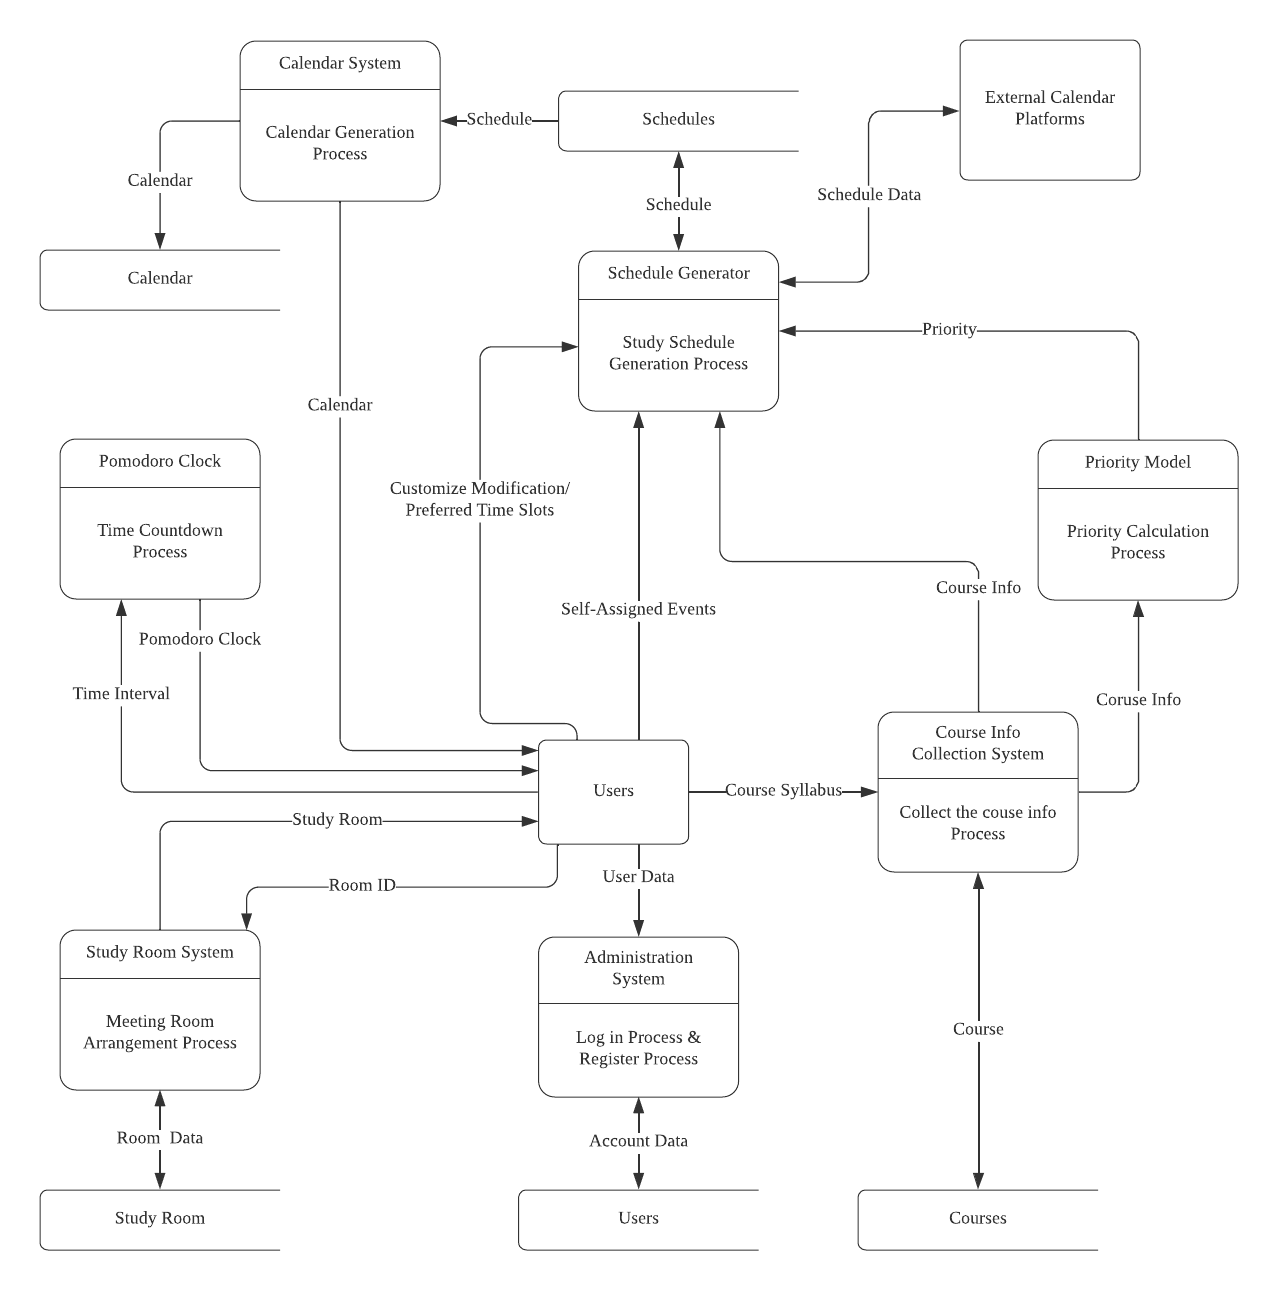
\includegraphics[width=0.8\textwidth]{DFD.png}
  \caption{Data Flow Diagram} 
  \label{fig:dfd} 
\end{figure}

\subsection{Data Dictionary}
\lips

\section{The Scope of the Product}
\subsection{Product Boundary}
\lips
\subsection{Product Use Case Table}
\lips
\subsection{Individual Product Use Cases (PUC's)}
\lips

\section{Functional Requirements}
\subsection{Functional Requirements}
\lips

\section{Look and Feel Requirements}
\subsection{Appearance Requirements}
\lips
\subsection{Style Requirements}
\lips

\section{Usability and Humanity Requirements}
\subsection{Ease of Use Requirements}
\lips
\subsection{Personalization and Internationalization Requirements}
\lips
\subsection{Learning Requirements}
\lips
\subsection{Understandability and Politeness Requirements}
\lips
\subsection{Accessibility Requirements}
\lips

\section{Performance Requirements}
\subsection{Speed and Latency Requirements}
\lips
\subsection{Safety-Critical Requirements}
\lips
\subsection{Precision or Accuracy Requirements}
\lips
\subsection{Robustness or Fault-Tolerance Requirements}
\lips
\subsection{Capacity Requirements}
\lips
\subsection{Scalability or Extensibility Requirements}
\lips
\subsection{Longevity Requirements}
\lips

\section{Operational and Environmental Requirements}
\subsection{Expected Physical Environment}
\lips
\subsection{Wider Environment Requirements}
\lips
\subsection{Requirements for Interfacing with Adjacent Systems}
\lips
\subsection{Productization Requirements}
\lips
\subsection{Release Requirements}
\lips

\section{Maintainability and Support Requirements}
\subsection{Maintenance Requirements}
\lips
\subsection{Supportability Requirements}
\lips
\subsection{Adaptability Requirements}
\lips

\section{Security Requirements}
\subsection{Access Requirements}
\lips
\subsection{Integrity Requirements}
\lips
\subsection{Privacy Requirements}
\lips
\subsection{Audit Requirements}
\lips
\subsection{Immunity Requirements}
\lips

\section{Cultural Requirements}
\subsection{Cultural Requirements}
\lips

\section{Compliance Requirements}
\subsection{Legal Requirements}
\lips
\subsection{Standards Compliance Requirements}
\lips

\section{Open Issues}
\lips

\section{Off-the-Shelf Solutions}
\subsection{Ready-Made Products}
\lips
\subsection{Reusable Components}
\lips
\subsection{Products That Can Be Copied}
\lips

\section{New Problems}
\subsection{Effects on the Current Environment}

\begin{itemize}
    \item The introduction of new time management tools may affect existing scheduling systems within educational organizations. Any changes to the way students manage the study schedule may affect the way teachers and administrators organize their workflow and thus their existing scheduling systems.

    \item The implementation of a new system may change the way students interact with existing tools and platforms. If the new tool enables seamless integration with existing popular scheduling platforms, users may stop using other scheduling tools. Some users may need to adapt to these changes, and this transition needs to be handled carefully to ensure a smooth user experience.

    \item The data security requirements of the new tool and the user access control may require changes to the current security infrastructure. Any potential impact on existing security protocols should be fully assessed, and measures taken to mitigate risks.

    \item The new system may change user workflows and procedures. If it automates and prioritizes tasks, this may impact the way they plan and manage assignment completion and course scheduling. Understanding and responding to these changes as early as possible is critical to ensure smooth operation.
\end{itemize}

\subsection{Effects on the Installed Systems}
This section specifies the interfaces between the new system and existing systems or components.
\begin{itemize}
    \item \textbf{Interface with Google Calendar}: The system should integrate with Google Calendar to synchronize and visualize task deadlines. The interface will involve certification, data exchange, and event management.
    
    \item \textbf{Interface with Outlook Calendar}: Similar to Google Calendar, the system shall integrate with Outlook Calendar to synchronize events. The interface will involve certification and event management.

    \item \textbf{Interface with Machine Learning Server}: The system relies on machine learning algorithms to prioritize tasks. This interface includes sending data to the machine learning server, processing suggestions, and integrating them into the user interface.

    \item \textbf{Interface to connect with users}: To facilitate collaborative learning, the system should enable users to connect with their peers. This interface includes user authentication, data exchange, and video chat integration.

    \item \textbf{Interface with videoconferencing hardware} Users will use webcams, microphones, and speakers for video chat during collaborative learning. This interface is required to access these hardware components and manage live video conferencing.
\end{itemize}
\subsection{Potential User Problems}
\begin{itemize}
    \item \textbf{User Confusion}:
    The addition of machine learning-driven task prioritization, facial recognition, and online collaborative learning session features may confuse or create resistance from some users who are unfamiliar with these concepts.
    
    \textbf{Prevention and mitigation measures:}
    \begin{itemize}
        \item Develop a user-friendly onboarding process and provide extensive training materials to ensure users can easily understand and use the new features.
        \item Provide customization options that allow users to customize the system to their preferences. This flexibility will help users take better control of their experience.
    \end{itemize}
    
    \item \textbf{Privacy Concerns}:
    Users may have privacy concerns, especially with attention-monitoring features such as facial recognition. They may be concerned that their facial data will be collected and used.
    
    \textbf{Prevention and Mitigation Measures:}
    \begin{itemize}
        \item Privacy concerns are addressed by implementing strong data protection measures. Users will be informed of what their data will be used for and how it will be processed and will be able to opt out of certain features.
    \end{itemize}
    
    \item \textbf{Technical Issues}:
    Technical issues or system incompatibilities may lead to adverse reactions, such as issues related to platform support or software bugs.
    
    \textbf{Prevention and Mitigation Measures:}
    \begin{itemize}
        \item Rigorous testing and quality assurance are conducted to detect and correct technical issues before they affect users. Updates and bug fixes will be performed regularly to ensure system stability.
    \end{itemize}
\end{itemize}

\subsection{Limitations in the Anticipated Implementation Environment That May
Inhibit the New Product}
\begin{itemize}
    \item The planned servers may not have enough processing power or storage capacity to handle the expected growth in users and data volume.
    
    \item Available network bandwidth may not be sufficient to support real-time videoconferencing for collaborative learning sessions, leading to potential performance issues.
    
    \item Implementing system integration with external calendaring platforms (e.g., Google Calendar, Outlook) takes into account that these platforms may have limitations or constraints that affect the quality of the integration.
    
    \item Hardware for facial recognition may not be readily available or may not meet the accuracy requirements for detecting the user's level of attention.
    
    \item The implementation environment may be subject to specific data privacy regulations that may affect the collection and storage of user data.
\end{itemize}

\subsection{Follow-Up Problems}
This section anticipates potential challenges, unintended consequences, and limitations that the project may encounter during development and implementation.

\begin{itemize}
    \item The implementation of new features or technologies in the system may inadvertently result in non-compliance with existing laws and regulations, such as user privacy protection aspect. The project team will conduct regular assessments. Any necessary changes will be made to address potential legal issues.
    \item 
\end{itemize}

\section{Tasks}
\subsection{Project Planning}
\href{https://github.com/wangq131/4G06CapstoneProjectT5/blob/main/docs/DevelopmentPlan/DevelopmentPlan.tex#L248C1-L265C6}{See Project Scheduling Section in Development Plan.}
\subsection{Planning of the Development Phases}
\href{https://github.com/wangq131/4G06CapstoneProjectT5/blob/main/docs/DevelopmentPlan/DevelopmentPlan.tex#L194C1-L245C16}{See Project Scheduling Section in Development Plan.}

\section{Migration to the New Product}
The project is a stand-alone application, not an upgrade or replacement of an existing product. There is no need to involve a product migration. The Migration to the New Product section is not needed.

\section{Costs}
The following are some of the major cost items that may need to be considered:

\begin{itemize} 
  \item \textbf{Cloud services}: using a cloud infrastructure (e.g. \textit{Amazon AWS}, \textit{Microsoft Azure}, or \textit{Google Cloud}) requires consideration of the cost of using cloud services.
  \item \textbf{Server hosting}: using an independent server, server hosting, and maintenance costs need to be considered.
  \item \textbf{Database}: database storage and access costs.
  \item \textbf{Data Backup}: regular data backup and storage costs.
  \item \textbf{Working Time}: takes NUMBER\_Of\_MEMBERS group members WORK\_HOURS a week.
\end{itemize}

\section{User Documentation and Training}
\subsection{User Documentation Requirements}
\lips
\subsection{Training Requirements}
\lips

\section{Waiting Room}
\lips

\section{Ideas for Solution}
\lips

\newpage{}
\section*{Appendix --- Reflection}

The information in this section will be used to evaluate the team members on the
graduate attribute of Lifelong Learning.  Please answer the following questions:

\begin{enumerate}
  \item What knowledge and skills will the team collectively need to acquire to
  successfully complete this capstone project?  Examples of possible knowledge
  to acquire include domain specific knowledge from the domain of your
  application, or software engineering knowledge, mechatronics knowledge or
  computer science knowledge.  Skills may be related to technology, or writing,
  or presentation, or team management, etc.  You should look to identify at
  least one item for each team member.
  \item For each of the knowledge areas and skills identified in the previous
  question, what are at least two approaches to acquiring the knowledge or
  mastering the skill?  Of the identified approaches, which will each team
  member pursue, and why did they make this choice?
\end{enumerate}

\end{document}